\onehalfspacing

\section{Motivation}

Im Zusammenhang mit der COVID-19-Pandemie erlebt Open Science seit 2020 enormen Aufschwung in der Wissenschaft. Deren Kerneigenschaften des ungehinderten kollaborativen Austauschs von Daten, Papers und Zwischenergebnissen werden eine entscheidende Rolle bei der raschen Impfstoffentwicklung zugewiesen. Vielfach wurde und wird daher die Bedeutung und Wirkung von Open Science gegenwärtig insbesondere im medizinischen und naturwissenschaftlichen Wissenschaftsbereich diskutiert.\footnote{Siehe zum Beispiel Lonni Besançon, Nathan Peiffer-Smadja, Corentin Segalas, Haiting Jiang, Paola Masuzzo, Cooper Smout, Eric Billy, Maxime Deforet, Clémence Leyrat: Open science saves lives: lessons from the COVID-19 pandemic, in: BMC Medical Research Methodology, Band 21, Artikelnr. 117, 2021, doi:10.1186/s12874-021-01304-y und CODATA Coordinated Expert Group (2020): Open Science for a Global Transformation. CODATA coordinated submission to the UNESCO Open Science Consultation, Zenodo, doi:10.5281/zenodo.3935461.} Die große Zahl an Open Science Initiativen zeigt zudem, dass Open Science in der Wissenschaft angekommen und in Begriff ist, sich dort zu etablieren. Im Kern geht es auch darum, die Integrität von wissenschaftlicher Forschung zu wahren, sie gerade im sogenannten postfaktischen Zeitalter zu stärken und sie somit weniger anfällig für Betrug und Fälschung in einer digitalen Welt zu machen.Auch auf gesellschaftspolitischer Ebene gewinnt Open Science an Relevanz. Die Europäische Union hat Open Science zu einem von insgesamt drei Grundsatzzielen für die Forschungsarbeit in Europa erklärt und die Deutsche UNESCO-Kommission hebt in ihrer Empfehlung von 2020 deren gesellschaftliche Bedeutung hervor:

\begin{quote}     
    ,,Darüber hinaus besteht mit Open Science eine Chance auf die praktische Umsetzung von seit Langem bestehenden politischen Forderungen: Mit Open Science kann Teilhabe an und Zugang zu wissenschaftlichen Erkenntnissen als Gemeingut und Menschenrecht praktisch umgesetzt werden, wie es bereits seit Ende des Zweiten Weltkriegs in der Allgemeinen Erklärung der Menschenrechte gefordert war.''\footnote{Deutsche UNESCO-Kommission e.V. (Hrsg.): Open Science. Perspektiven aus Deutschland auf die Erarbeitung der geplanten Empfehlung der UNESCO. UNESCO recommendation on Open Science, Berlin 2020, S. 8.}    
\end{quote}

In der Konsequenz stellt sich auch für die Geschichtswissenschaften die Frage, einserseits welche Wirkung Open Science auf die historische Forschung und andererseits welche Wirkung historische Forschung mit Open Science entfalten kann. Hierauf möchte die Arbeit Antworten finden, indem am Beispiel eines geschichtswissenschaftlichen Forschungsfelds die praktische Umsetzung von Open Science untersucht wird. Damit trägt sie zum Anschluss der Geschichtswissenschaften an gegenwärtig aktuelle wissenschaftliche Debatten bei und kann neue Wege in der digitalen Welt für die historische Forschung explorieren. 

\section{Zielsetzung}

Ausgehend von Forschungsdaten zu Jüdischen Gewerbebetrieben soll erstmals überhaupt ein gesamtheitliches Forschungsdatenmanagement für diese entwickelt werden. Der Fokus liegt dabei auf Studien, die systematisch Daten zu Jüdischen Gewerbebetrieben zum Zwecke der Erkenntnisgenerieung gesammelt haben. In das Forschungsdatenmanagement sollen Open Science-Ansätze integriert und im Zuge dessen die Implementierbarkeit sowie der Nutzen für die historische Forschung ausgelotet werden. Ziel ist es, am Ende ein prototypisches Konzept zu offenem Forschungsdatenmanagemet mit Open Science-Bezug vorliegen zu haben, das auch für andere historische Felder insbesondere der Zeitgeschichte übertragbar und nutzbar wäre.

\section{Methodisches Vorgehen}

Bei der Konzeption eines Forschungsdatenmanagements wird sich an etablierte softwaretechnische Verfahren orientiert. Im Kern basiert es auf einer Anforderungsanalyse, wie sie auch im Software-Engineering verwendet wird.\footnote{Siehe zum Beispiel M. Broy, M. Kuhrmann: Anforderungsanalyse und Anforderungsmanagement, in: Einführung in die Softwaretechnik, Berlin, Heidelberg 2021, S. 199-222, doi:10.1007/978-3-662-50263-1\_5.} Sie dient der Festlegung und Bewertung von Anforderungen im Softwareentwicklungsprozess. Mit ihr soll das Risiko gesenkt werden, eine fehlerhafte oder an den Nutzerbedürfnissen vorbei entwickelte Software auszuliefern. Die Anforderungsanalyse wird daher als ein wesentlicher Qualitäts- und Erfolgsfaktor bewertet.

\begin{figure}[h]
    \centering
    \frame{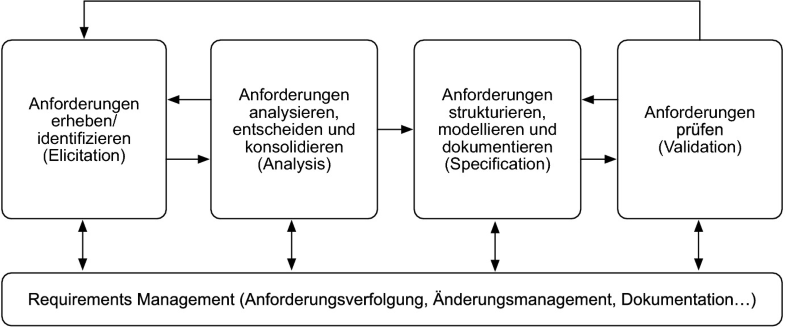
\includegraphics[scale=0.4]{Anforderungsanalyse}}
    \caption{Prozess der Anforderungsanalyse.}
    \label{fig:anforderungsanalyse}
\end{figure}

Wie aus Abbildung \ref{fig:anforderungsanalyse} hervorgeht, ist der Arbeitsprozess der Anforderungsanalyse iterativ und inkrementell. Dies kann in dieser Arbeit nur teilweise umgesetzt werden. Insbesondere die sich wiederholenden Vorgänge dienen dazu, Anforderungen regelmäßig zu überprüfen und letztlich damit einen Entwurf in ein finales Softwareprodukt zu überführen. Diese Aufgabe erfordert ein begleitendes Management (Requirements-Management), da es hier von der konzeptuellen Arbeitsphase in die Organisations- sowie Realisierungsphase geht. Die Konzeption eines offenen Forschungsdatenmanagements bildet hier nur die erste konzeptuelle Phase im Entwicklungsprozess ab. Für die nächsten Schritte der Implementierung wären über die Arbeit hinaus Ressourcen notwendig.  

Mit Open Science und Forschungsdatenmanagement als Rahmenbedingungen von offenem Forschungsdatenmanagement werden im ersten Kapitel die Grundlagen herausgearbeitet und der Forschungsstand überblickt, der den gegenwärtigen Ist-Stand von Umsetzungsmöglichkeiten vor allem auf der technischen Ebene aufzeigt. Im zweiten Kapitel wird zuerst die inhaltliche Einordnung der Forschungsdaten zu Jüdischen Gewerbebetrieben in das Forschungsfeld zur Vernichtung der wirtschaftlichen Existenz der Juden im Nationalsozialismus vorgenommen. Daran anknüpfend werden inhaltliche Kriterien entwickelt, die das \textit{offene} Forschungsdatenmanagement im Kontext des Forschungsfelds klar definieren und dessen Leistungsumfang grundlegend abstecken. Anschließend wird sich mit weiteren Voraussetzungen, die das offene Forschungsdatenmanagement parametrisieren, auseinandergesetzt. Dazu gehören die Interessengruppen (Stakeholder), die grundsätzliche Bereitschaft zu Open Science sowie die rechtlichen und ethischen Rahmenbedingungen. Zur Identifizierung der Interessengruppen (Stakeholder) sowie zur Erhebung der forschungsfeldspezifischen Anforderungen wurden vier Experteninterviews durchgeführt und mit basalen qualitativen inhaltsanalytischen Techniken in einem Mix-Method-Verfahren ausgewertet. Hierbei erfolgte anhand eines Fragenkatalogs eine deduktive Hauptkategorienbildung, welche durch induktiv gebildete Subcodes ergänzt wurde.\footnote{Das Codesystem und die Transkripte sind im Anhang D.4 beigefügt.} Abschließend wird eine prototypische Lösung des offenen Forschungsdatenemanagements am Beispiel der Forschungsdaten zu Jüdischen Gewerbebetrieben entwickelt. Hierbei wird der gewählte Lösungsansatz diskutiert bevor im nächsten Schritt das offene Forschungsdatenmanagement an einem idealtypischen Forschungsprozess entlang strukturiert, modelliert und dokumentiert wird.\\ \\
Im Sinne ihres Themas wurde die Arbeit offen erarbeitet und ist auf der \textit{Open Science Framework}-Plattform vollumfänglich zugänglich.\footnote{Weitere Ausführungen dazu im Anhang D.1.}

